\documentclass[times, utf8, zavrsni]{fer}

\usepackage{booktabs}
\usepackage[hidelinks]{hyperref}
\usepackage{float}

\begin{document}

\thesisnumber{000}
\title{Klasifikacija uporabom umjetnih neuronskih mreža}
\author{Darijo Brčina}

\maketitle

% Ispis stranice s napomenom o umetanju izvornika rada. Uklonite naredbu \izvornik ako želite izbaciti tu stranicu.
\izvornik

% Dodavanje zahvale ili prazne stranice. Ako ne želite dodati zahvalu, naredbu ostavite radi prazne stranice.
\zahvala{}

\tableofcontents

\chapter{Uvod}
Uvod rada. Nakon uvoda dolaze poglavlja u kojima se obrađuje tema.

\chapter{Pregled područja}
Pitate li se ikada što je to inteligencija te čemu nam služi. To pitanje postavljeno je još za vrijeme začetka filozofije kao znanosti kada su se tadašnji filozofi pitali kako i na koji način je ljudsko razmišljanje, učenje i pamćenje ostvareno. Ni dan danas ne postoji jednoznačan odgovor na to pitanje jer ljudski mozak i dalje predstavlja jednu veliku nepoznanicu koja vjerojatno nikada ili ne tako skoro neće biti razriješena. No znanost je podosta napredovala i shodno tomu se razvila želja da se ljudska inteligencija pokuša pretočiti u nekakvu vrstu inteligencije strojeva.

Početak ovakvog razmišljanja datira od 50-tih godina dvadesetog stoljeća kada Alan Turing u članku \textit{Computing Machinery and Intelligence} časopisa \textit{Mind} postavlja pitanje: Mogu li strojevi misliti? \engl{Can machines think?} na koje pokušava odgovoriti kroz tzv. igru imitacije \engl{imitation game}. Sudionici igre su tri igrača: igrač A, igrač B i igrač C gdje su igrači A i B ispitanici a igrač C ispitivač. Cilj igrača C je utvrditi spol ispitanika postavljanjem pitanja, cilj igrača B je pomoći ispitivaču C a cilj igrača A je navesti ispitivača C na pogrešnu identifikaciju. Što će se dogoditi ako stroj uzme mjesto igrača A? Ako broj pogrešaka igrača C bude gotovo jednak u oba slučaja, onda je stroj inteligentan. \citep{turingAI}. Ovakav princip se često naziva turingov test \engl{Turing test}.

1956. se održava konferencija u Dartmouthu \citep{wiki:DART} na inicijativu John McCarthy-a, tadašnjeg mladog profesora matematike na fakultetu u Dartmouthu, koji okuplja oko sebe nekolicinu znanstvenika i prijatelja kako bi pokušali koncepte ljudske inteligencije preslikati u inteligenciju strojeva. Cilj je pokazati kako strojevi koriste jezik, kako zaključuju i stvaraju apstraktne koncepte i kako vremenom postaju sve prilagodljiviji na predočene probleme baš kao i ljudi. Inicijalna ideja je bila da se neki od navedenih problema može dokazati uz manju skupinu dobrih znanstvenika i kroz period od jednog ljeta (McCarthy et al. 1955). To naravno nije bilo moguće. Time se formalno uvodi pojam \textit{umjetna inteligencija}.

\section{Umjetna inteligencija}
Kao što je anticipirano ranije, umjetna inteligencija \engl{artificial intelligence} je laički rečeno inteligencija strojeva a znanost koja se jednim dijelom bavi proučavanjem umjetne inteligencije jest računarska znanost \engl{computer science}.

Primjena umjetne inteligencije danas je izrazito rasprostranjena kroz gotovo svaku industriju. Pronalazimo ju u medicini, automobilskoj industriji, robotici, pa i u sportskoj i industriji igara. Jedan od poznatijih događaja koji prikazuje primjenu umjetne inteligencije dogodio se 2016. kada je računalo naziva \textit{AlphaGo} u igri \textit{Go} uspijelo pobijediti svjetskog prvaka Lee Sedolu rezultatom 4:1 te time ostvario velik uspjeh u svijetu umjetne inteligencije kao i pažnju javnosti \citep{moyerGO}.

Umjetnu inteligenciju je dakako potrebno trenirati i učiti pa je tako učenje podijeljeno na dvije veće cjeline:
\begin{center}
    \begin{enumerate}
        \item simboličko učenje te
        \item strojno učenje.
    \end{enumerate}
\end{center}

\subsection{Simboličko učenje}
Simbolička umjetna inteligencija \engl{symbolic artificial intelligence} je izraz koji definira skup istraživačkih metoda koje se temelje na ljudima lako čitljivim simbolima \engl{human-readable simbol} koji modeliraju probleme i logiku. Jedan od najboljih primjera jesu \textit{ekspertni sustavi} koji se temelje na skupu pravila. Pravila su modelirana na sličan način kao i Ako-Onda rečenica \engl{If-Then statement} koja je u ljudskoj komunikaciji svakodnevno u upotrebi. Također, razne vrste logika poput propozicijska \engl{Propositional logic}, često referirana kao Boolova algebra, logika prvog reda \engl{First order logic}, poznatija kao predikatna logika \engl{Predicate logic}, neizrazita logika \engl{Fuzzy logic} pripadaju upravo simboličkoj umjetnoj inteligenciji. Ovakav način učenja bio je popularan početkom 1950. sve do kraja 1980 \citep{wiki:SIMB}.

\subsection{Strojno učenje}
Strojno učenje \engl{machine learning, ML} predstavlja niz metoda i algoritama koji sustavima pružaju stjecanje novog znanja kroz modeliranje obrazaca koje onda kasnije mogu iskoristiti za predviđanje novih podataka ili sličnih \citep{cupicML}. Glavna ideja je da sustavi uče iz iskustva, empirijski, bez da se programska implementacija mijenja što znatno olakšava manipulaciju istih.

Danas postoji nezgrapno puno podataka koje je moguće i koje je potrebno iskoristiti za učenje pa je cilj konstruirati sustave koji mogu iskoristiti baš te podatke za neka korisna ponašanja poput predviđanja i raspoznavanja raznih uzoraka \citep{cupicML}. Podatci se svrstavaju u dvije grupe: \textit{numerički} i \textit{kategorički} podatci. Numerički podatci su svi oni podatci nad kojima je moguće izvršiti aritmetičke operacije. Npr. unos dnevnih kalorija, broj slobodnih bacanja na košarkaškoj utakmici, isplata plaća i sl. Kategorički podatci se dodatno dijele u dvije podgrupe: nominalni i ordinalni podatci. Nominalni podatci su imenovani podatci koji nisu numerički, tj. podatci nad kojima nisu definirane aritmetičke operacije. Npr. podatci o spolu jedinke, osjećaju raspoloženja poput "tužan" ili "veseo" i sl. Ordinalni podatci također nemaju definiranu aritmetiku, no imaju definiran prirodan poredak i mogu se uspoređivati. Npr. mišljenje jedne osobe može biti "jako zadovoljan" dok druge "zadovoljan" što možemo usporediti i konstruirati prirodan poredak.

Strojno učenje dijelimo na četiri područja:
\begin{center}
    \begin{enumerate}
        \item nadzirano učenje,
        \item nenadzirano učenje,
        \item polu-nadzirano učenje te
        \item podržano učenje.
    \end{enumerate}
\end{center}

\textit{Nadzirano učenje} je tema ovog rada pa će biti obrađeno detaljnije u narednom poglavlju.

\bigskip

\textit{Nenadzirano učenje} \engl{unsupervised learning} je vrsta učenja u kojem skup podataka predstavljaju samo ulazni podatci bez znanja o tome kako bi isti trebali biti tabelirani. Zbog ovakvog pristupa, učenje je i dobilo ime nenadzirano učenje, tj. učenje bez prisustva učitelja \engl{supervisor}. Najpoznatiji postupak nenadzirano učenja je postupak grupiranja \engl{clustering}. Cilj grupiranja je na temelju danih podataka pokušati pronaći sve podatke koji imaju slična svojstva te ih zatim grupirati u odvojene razrede. Npr. neka skup ulaznih podataka sustava bude mješavina slika ljudi i slika automobila. Kao konačni rezultat, moraju se stvoriti dva razreda: razred ljudi te razred automobila. Na \ref{fig:clustering} možete vidjeti primjer grupiranja.

\begin{figure}[H]
    \centering
    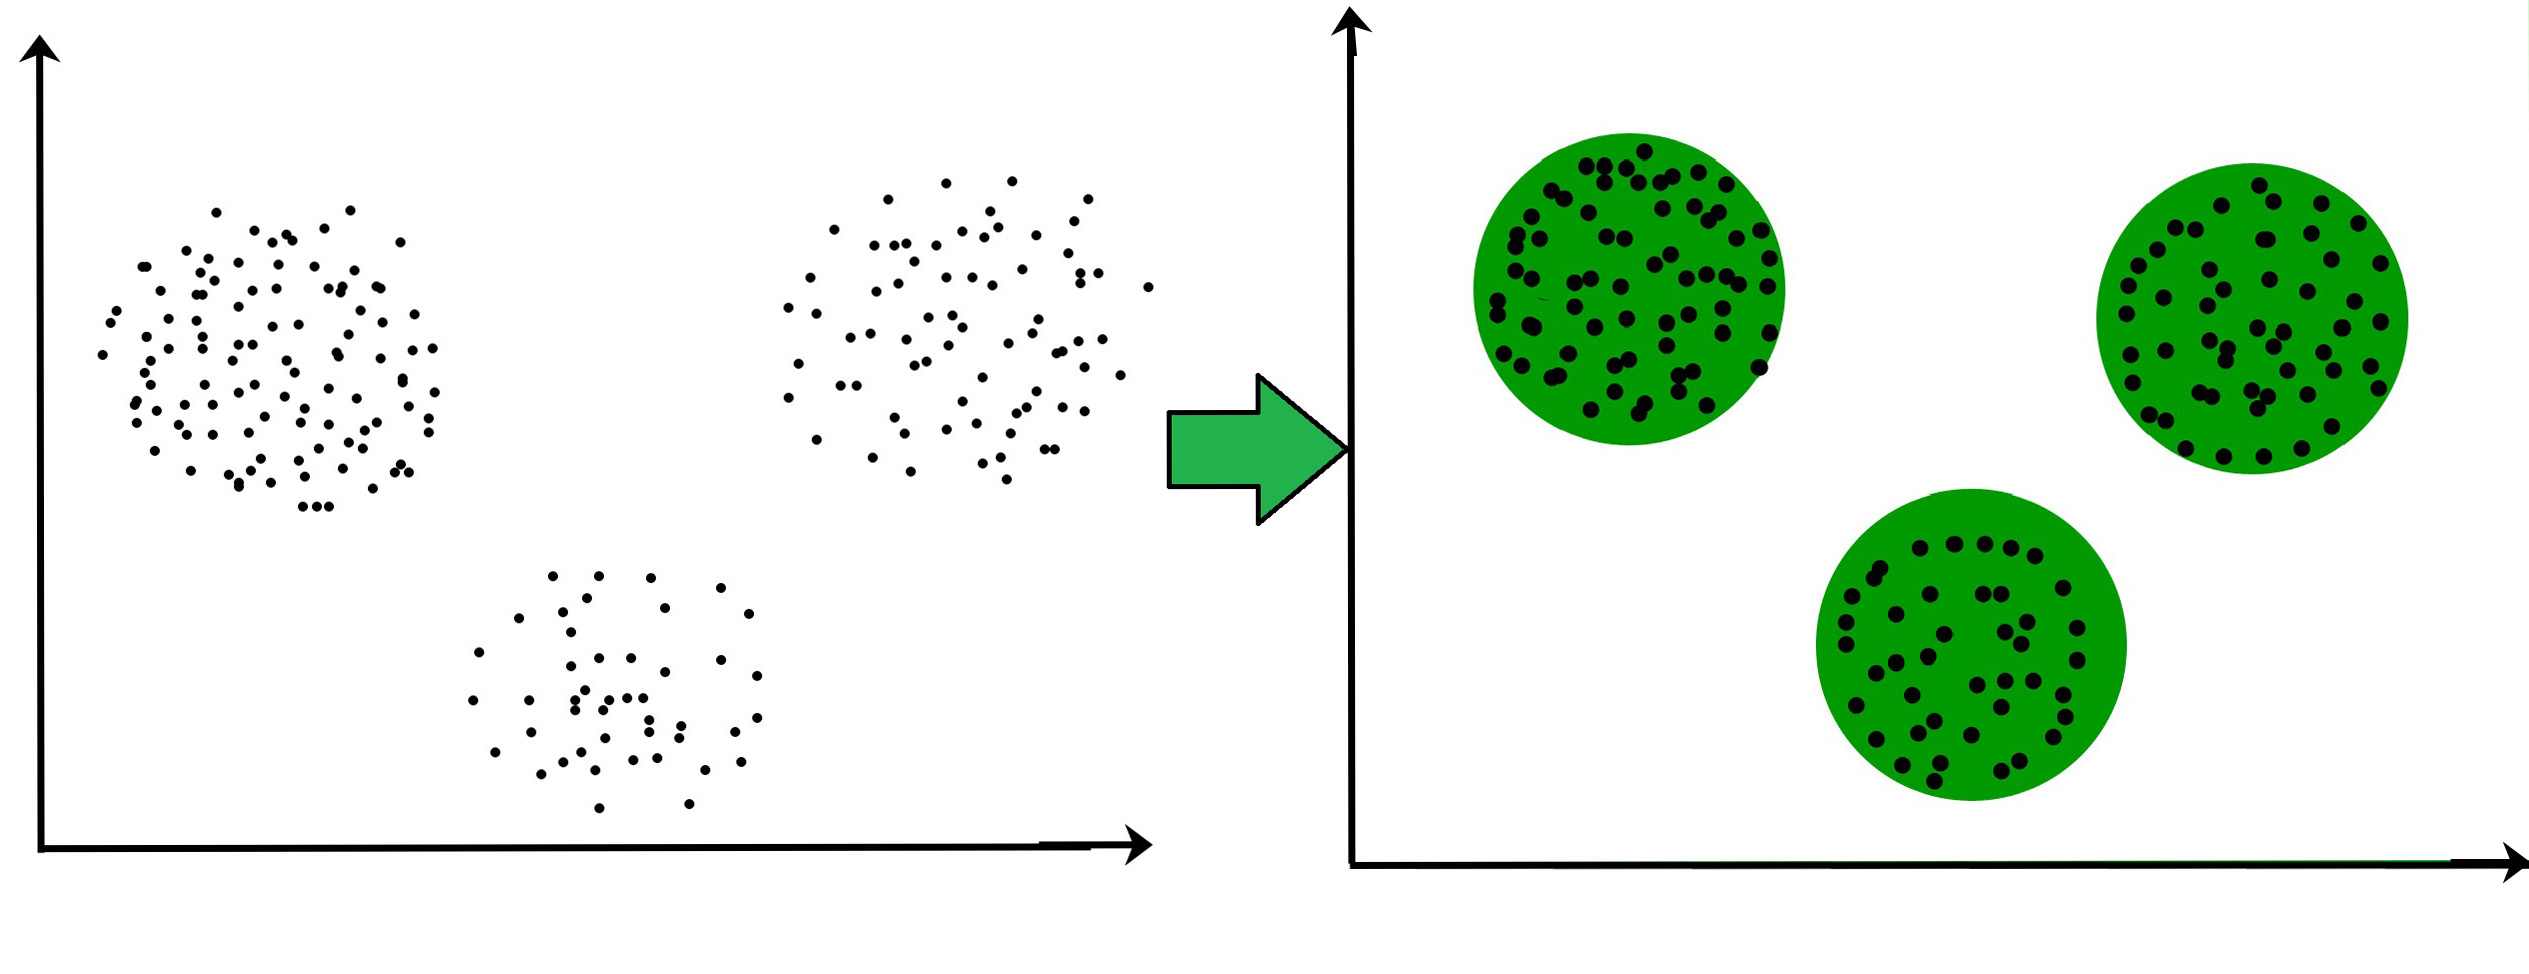
\includegraphics[scale=0.35]{img/clustering.jpg}
    \caption[Caption for LOF]{Primjer grupiranja\footnotemark}
    \label{fig:clustering}
\end{figure}
\footnotetext{Preuzeto sa https://www.geeksforgeeks.org/clustering-in-machine-learning/}

Uz grupiranje poznati postupci su i postupci smanjenja dimenzionalnosti \engl{dimensionality reduction}, postupci otkrivanja stršećih ili novih vrijednosti \engl{outlier detection, novelty detection} i drugi.

\bigskip

\textit{Polu-nadzirano učenje} \engl{semi-supervised learning}, kao što samo ime nalaže, je učenje u kojem se isprepliću koncepti nadzirano učenje sa konceptima nenadziranim učenjem. Ono pokazuje dosta veće uspjehe nego navedeni, no izrazito je zahtjevnija izvedba \citep{wiki:SEMISUP}.

\bigskip

\textit{Podržano učenje} \engl{reinforcement learning, RL} je vrsta učenja koja se potpuno razlikuje od svih do sada navedenih jer ono ne očekuje nikakve tabelirane ulazne ili izlazne podatke već je glavna ideja optimizacija ponašanja računalnih agenata. Razmatra se interakcija agenta sa okolinom \engl{environment} kroz niz akcija za koje isti može biti nagrađen ili kažnjen ovisno o ishodu akcije. Željeni cilj agenta je maksimizirati mogući dobitak nagrade. Na slici \ref{fig:reinforcement-learning} je jasno prikazan sustav agenta.

\begin{figure}[H]
    \centering
    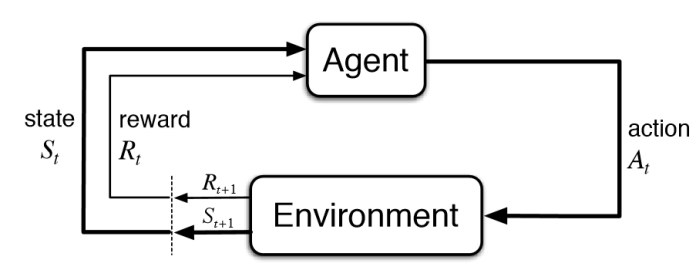
\includegraphics[scale=0.7]{img/reinforcement-learning.jpg}
    \caption[Caption for LOF]{Dijagram podržanog učenja\footnotemark}
    \label{fig:reinforcement-learning}
\end{figure}
\footnotetext{Preuzeto sa https://www.kdnuggets.com/2018/03/5-things-reinforcement-learning.html/}

\chapter{Nadzirano učenje}

\chapter{Zaključak}
Zaključak.

\bibliography{literatura}
\bibliographystyle{fer}
\nocite{*}

\begin{sazetak}
Sažetak na hrvatskom jeziku.

\kljucnerijeci{Ključne riječi, odvojene zarezima.}
\end{sazetak}

\engtitle{Classification Based on Artificial Neural Networks}
\begin{abstract}
Abstract.

\keywords{Keywords.}
\end{abstract}

\end{document}
